\documentclass[oneside,12pt]{Classes/aesm_edspia}

\usepackage{minitoc}
\usepackage[latin1]{inputenc}
\usepackage[english,french]{babel}
\usepackage[T1]{fontenc}
\usepackage{amsmath}
\usepackage{lmodern}%font modern
\rmfamily
\DeclareFontShape{T1}{lmr}{bx}{sc}{<->ssub * cmr/bx/sc}{}
\usepackage{lettrine}
\usepackage{tabularx}
\usepackage{epsfig, floatflt, amssymb}
\usepackage{moreverb} %% pour le verbatim en boite
\usepackage{cases}%equations en systemes numerotes - soluce possible package : CASES
\usepackage{multirow} %% pour regrouper un texte sur plusieurs lignes dans une table
\usepackage{url} %% pour citer les url par \url
\usepackage[all]{xy} %% pour la barre au dessus des symboles
\usepackage{textcomp} %% pour le symbol pour mille par \textperthousand et degres par \degres
\usepackage[right]{eurosym}
\usepackage{setspace} %interligne simple, double etc...
\usepackage{Classes/eurosans} %%pour le symbole \euro
\usepackage{epic,eepic}
\usepackage{soul}
\usepackage[nottoc]{tocbibind} % tables des figures, des matieres et autres dans la TOC
\usepackage{fancybox}
\usepackage[leftcaption]{sidecap}
\usepackage[labelsep=endash, textfont={footnotesize, singlespacing}, margin=10pt, format=plain, labelfont=bf]{caption}
\usepackage[Conny]{Classes/fncychap} %en tete chapitrage
\newcommand{\ie}{c.-\`a-d.~}
\hbadness=10000% pb d'overfull box regle
\hfuzz=50pt
\pdfcompresslevel9 % pour compresser le pdf final au maximum
\pdfoptionpdfminorversion=5 % pour accepte les images PDF version 1.5 (ex: celles produites par Office 2007)
\def\underscore{\char`\_}
\makeatletter
\renewcommand{\thesection}{\arabic {section}}
\renewcommand{\SC@figure@vpos}{c}% centrer verticalement le caption avec le package sidecap...
\renewcommand{\fnum@figure}{\small\textbf{Figure~\thefigure}}
\renewcommand{\fnum@table}{\small\textbf{Tableau~\thetable}}

\makeatother
\usepackage{subfig}
\def\thechapter{\Roman{chapter}}

%\usepackage[framed,numbered,autolinebreaks,useliterate]{Classes/mcode}


%%% Listings

\usepackage{listings}
\lstloadlanguages{xml, java}

	 \usepackage{listings}
  \usepackage{courier}
 \lstset{
         basicstyle=\footnotesize\ttfamily,
         %numbers=left,
         numberstyle=\tiny,
         %stepnumber=2,
         numbersep=5pt,
         tabsize=2,
         extendedchars=true,
         breaklines=true,
         keywordstyle=\color[rgb]{0.43,0,0}\textbf,
    		frame=b,
         commentstyle=\color[rgb]{0.51,0.51,0.51} \textit ,
         stringstyle=\ttfamily  \color[rgb]{0,0.44,0} ,
         showspaces=false,
         showtabs=false,
         xleftmargin=17pt,
         framexleftmargin=17pt,
         framexrightmargin=5pt,
         framexbottommargin=4pt,
         %backgroundcolor=\color{lightgray},
         showstringspaces=false
 }

 \usepackage{caption}
\DeclareCaptionFont{white}{\color{white}}
\DeclareCaptionFont{red}{\color{red}}
\DeclareCaptionFont{black}{\color{black}}
\DeclareCaptionFormat{listing}{\colorbox[cmyk]{0.43, 0.35, 0.35,0.01}{\parbox{\textwidth}{\hspace{15pt}#1#2#3}}}
\captionsetup[lstlisting]{format=listing,labelfont=black,textfont=white, singlelinecheck=false, margin=0pt, font={bf,footnotesize}}


%%%%%%%%%%%%%%%%%%%%%%%%%%%%%%%%%%%%%%%%%%%
\begin{document}
%%%%%%%%%%%%%%%%%%%%%%%%%%%%%%%%%%%%%%%%%%%
\renewcommand\figurename{\small\textbf{Figure}}

\addtocounter{page}{-1}%pour revenir e 0

% Pour remplir la page de garde
\AuteurA{Marouane} {ELKAMEL}
%\AuteurB{Flen2} {FOULENI}
%\AuteurC{Flen3} {FOULENI}
%\AuteurD{Flen4} {FOULENI}
\Encadrant{Mr}{Aymen}{SELLAOUTI}
\EncadrantS{Mr} {Anis} {KALLEL}

\Filiere{GL}
\datesout{--/--/2019}



\President{M. President} {FLEN}     %% President du Jury
\RapporteurA{Mme. Rapporteur} {FLENA} %%Rapporteur



\AnneeUniv{2018/2019}

%%%%%%%%%%%%%%%%%%%%%%%%%%%%%%%%%%%%%%%%%%%
\makethese %% cree la couverture.

\onehalfspacing

% une page blanche (deuxieme de couverture)
\newpage\thispagestyle{empty}\addtocounter{page}{-3}
\null\newpage\thispagestyle{empty}


\frontmatter %numerotation en iii
\pagestyle{fancy}
\fancyhf{}
\fancyhead[R]{Remerciements}
\fancyfoot[R]{\thepage}
\renewcommand{\headrulewidth}{0.5pt}
\renewcommand{\footrulewidth}{0pt}

\chapter*{Dedication}
%===================================================================

I couldn't be the person I am today or accomplish anything in my life, including this project, without the help of everyone who has believed in me from day one, especially :\newline


My mother \textbf{Salwa}, who dedicated her life to my sisters and I's success. She has sheltered us from anything that could've stopped us from achieving our goals.\newline

My father \textbf{Rafik},  who has made our lives feel so comfortable and easy throughout the years. He has never hesitated to handle all life's hardships without ever letting trouble reach our home.\newline

My Aunt \textbf{Salma}, for taking me under her wing from the day I moved to Tunis and treating me as a son amongst her children.\newline

My \textbf{family}, for being the greatest people to grow up around, teaching me the most important life lessons and creating the best possible environment to become someone who would make them proud.\newline

My \textbf{friends}, for inspiring me throughout all these years and for being the support and motivation that has gotten me to this next step in my life. I couldn't be here without each and every one of you, and I'll always be there for you.\newline

\begin{center}
	\textbf{To everyone who is special to me, I dedicate this work}
\end{center}

\chapter*{Acknowledgments}

This work would not have been possible without the valuable cooperation of a number of people I would like to pay tribute to.\newline

I would like to thank all those who have made this internship a rewarding and enjoyable experience, especially :\newline

\textbf{Mr. Nebras JEMEL}, co-founder and CEO of Flouci, for believing in me from day one, my internship tutor \textbf{Mr. Anis KALLEL}, co-founder and CTO, who introduced me to the team and helped me greatly throughout my journey. Thank you for your advice and guidance throughout this internship. \newline

The \textbf{"Flouci"} team, my second family, for their support and direction. More importantly, their devotion and passion for what we are doing inspires me every day.\newline

I would especially like to thank my supervisor \textbf{Mr. Aymen SELLOAUTI} for his availability, remarks, and advice. I also would like to express my respect and my gratitude to him.\newline

Finally, I also express my sincere appreciation to the members of the jury : \textbf{Mr Flen} and \textbf{Mr Flen} for accepting to evaluate my work.


%%%%%%%% TOC

%profondeur dans la Table of Contents et de la numerotation des sections

\setcounter{secnumdepth}{3}
\setcounter{tocdepth}{3}


\renewcommand{\contentsname}%
    {Table of Contents}%

%%%%minitoc
\dominitoc % genere la minitoc
\nomtcrule % supprime les lignes horizontales de la minitoc
\renewcommand{\mtctitle}{Plan} % Modifie le titre de la minitoc

%%%%
\tableofcontents

\renewcommand{\headrulewidth}{0.5pt}
\renewcommand{\footrulewidth}{0pt}
\fancyhead[R]{Table of Contents}


%%%%%%%% Figures

\makeatletter
%\renewcommand{a\thefigure}{\@arabic\c@figure}
\@addtoreset{figure}{chapter}
\makeatother

\renewcommand{\headrulewidth}{0.5pt}
\renewcommand{\footrulewidth}{0pt}
\renewcommand\listfigurename{List of Figures}
\listoffigures \mtcaddchapter

\fancyhead[R]{List of Figures}
\newpage


%%%%%%%% Tableaux

\makeatletter

\renewcommand{\headrulewidth}{0.5pt}
\renewcommand{\footrulewidth}{0pt}
\renewcommand\listtablename{List of Tables}

\listoftables  \mtcaddchapter

\fancyhead[R]{List of Tables}

%%%%%%%%%%%%%%%%%%%%%%%%%%%%%%%%%%%
%\fancyhead[R]{Resumes}

\chapter*{Summary}
\addcontentsline{toc}{chapter}{Summary}
%===================================================================

Brief summary \dots


%%%%%%%%%%%%%%%%%%%%%%%%%%%%%%%%%%%


\mainmatter %numeros arabes
\pagestyle{fancy}
\fancyhead[R]{Introduction Generale}
\chapter*{General Introduction}
\graphicspath{{Introduction/figures/}}
\addcontentsline{toc}{chapter}{General Introduction}
\begin{spacing}{1.2}
%==================================================================================================%

In the modern software world APIs are becoming a must for every tech company to allow products to be integrated by developers in multiple Apps.

APIs do all this by "exposing" some of a product's internal functions to the outside world in a limited fashion. That makes it possible for applications to share data and take actions on one another's behalf without requiring developers to share all of their software's code. 



\begin{figure}[!ht]\centering
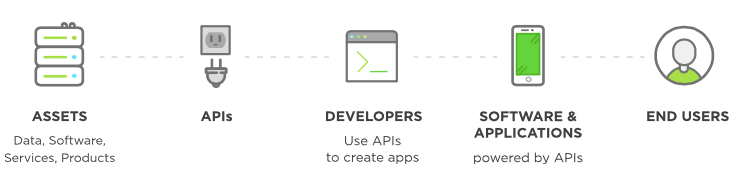
\includegraphics[scale=0.6]{API.png}
\caption{APIs }
\label{fig:fig1}
\end{figure}

That's the reason why KAOUN, a Tunisian FinTech start-up, decided to create its own developers API for its main product FLOUCI which is a mobile payment solution. This project will expand FLOUCI to the developers world and unleash the full potential of the product, also it could take FLOUCI into new markets and open doors for unlimited integrations.\newline


The following report is a synthesis of the efforts done to build FLOUCI developers API.

 To detail the process of our work, we have divided this report into XX chapters representing the different aspects of our project.

In the first chapter, entitled Project scope, we started with a presentation of the host company. Afterwards, we gave an overview of our project and we detailed the followed methodology for its realization.


The second chapter is about the development disciplines and rules we set during our project development life cycle. It's a detailed explanation of the development practices needed to start our project development in the most efficient way possible. 



We close our work with a general conclusion in which we try to evaluate our contribution as well as we develop our vision for the project's potential improvements.




\end{spacing}

\fancyhf{}
\fancyhead[R]{Introduction Generale}
\fancyfoot[R]{\thepage}
\renewcommand{\headrulewidth}{0.5pt}
\renewcommand{\footrulewidth}{0pt}



\setcounter{chapter}{0} %indique le numero reel du chapitre, pour la mini Table of Contents
\chapter{Project Scope}
\adjustmtc
\minitoc  %insert la minitoc

\graphicspath{{Chapter1/figures/}}
%==============================================================================
\pagestyle{fancy}
\fancyhf{}
\fancyhead[R]{\bfseries\rightmark}
\fancyfoot[R]{\thepage}
\renewcommand{\headrulewidth}{0.5pt}
\renewcommand{\footrulewidth}{0pt}
\renewcommand{\chaptermark}[1]{\markboth{\MakeUppercase{\chaptername~\thechapter. #1 }}{}}
\renewcommand{\sectionmark}[1]{\markright{\thechapter.\thesection~ #1}}

\begin{spacing}{1.2}
%==============================================================================

\section*{Introduction}
This chapter is dedicated to the presentation of our project's general scope.
This will include an introduction of the host company Kaoun and it's main product Flouci. Also, we will give an overview of the developer API project. After that, we will describe the chosen methodology that we followed during the realization of our project.
\section{Host company presentation}
In The first section of the report, we will introduce Kaoun, The host company that made the project possible.
\subsection{Presentation of Kaoun}
\begin{center}
	
\includegraphics[scale=0.2]{kaounlogo.png}
\end{center}



Kaoun is a new FinTech company that builds reliable infrastructure for payments and credits in Tunisia, and whose mission is to enable all individuals and businesses to access financial services using any phone, anywhere, anytime.

Kaoun's first product, Flouci, is a mobile and web payment application built on top of a unique decentralized inter and intrabank infrastructure that allows instant transactions for peer to peer transfers and merchant payments. Kaoun plans to work with governments, traditional banks, mobile operators, and microfinance institutions to fix the lag between technology adoption and financial inclusion by reducing the barriers to entry for the unbanked and the underbanked.








\subsection{Presentation of Flouci}
\begin{center}
	
\includegraphics[scale=0.2]{floucilogo.png}
\end{center}
Flouci is the first wallet designed to innovate mobile payment in Tunisia. It serves as a quick, easy, and convenient way to open a bank account, send and receive money, and pay different merchants in-person or online, all from within the app.
\begin{itemize}
  \item \textbf{Open an account:}

  In order to create a Flouci account, you either link your Flouci wallet to an existing bank account or follow the step-by-step KYC (Know Your Customer) guide to create an account with one of our partner financial institutions. Once you have your wallet and your QR code, you can start sending and receiving money and paying merchants using your phone.

  \item \textbf{Send and receive money:}

  Once you create a Flouci account, you can send and receive money to and from anybody that has a flouci account/wallet. It's easy, cheap, and secure. And the best part is that it's practically instant. All you have to do is enter their number or scan their personal QR code to access their profile. You then enter the amount and confirm. You both then receive a confirmation SMS and you're done.
  \item \textbf{Pay merchants:}

  Through Flouci, you have access to a wide range of partner merchants across Tunisia. You can pay through the app by just scanning the QR code shown on the counter of the merchant. No waiting lines, no more looking for change or realizing you forgot your wallet at home.
\end{itemize}

\section{Project overview}
In this section, we will start by presenting the developers API project context, then we will set our project goals.
\subsection{Project Context}
Flouci in its first version made it possible for users to pay merchants in simple steps and without the need of cash.
Flouci main app made it easy to transfer money between accounts. With the use of QR codes, users can send and receive money in less than 5 seconds.

\subsection{Flouci limitations}
The market is rapidly shifting toward online e-commerce sites with companies like Jumia, Tayara and many other introducing their solutions in Tunisia.

In its current implementation, Flouci is not able to integrate into any form of online payments due to the lack of its implementation.

Facing this problem and a fast moving e-commerce market the company had to move toward implementing a solution for developers.

The API should make it possible for developers to link their Flouci wallets to their e-commerce sites and add Flouci as an easy and instant payment method.
\subsection{Project goals}
To bring developers to the Flouci world and allow e-commerce owners to introduce a mobile payment solution Kaoun has decided to build its own developer API from scratch and provide an easy way to accept payments in few simple steps. This presented the opportunity for us to turn this problem into the main objective of our graduation project.

By the end of our project, we need to achieve these goals :
\begin{itemize}
  \item \textbf{Create Account:}
  Any developer should be able to create a Flouci developer account from the web platform, basic information is needed to open an account.

  Also, it should be possible to use an existing Flouci account and switch it to developer mode.
  \item \textbf{Create App and link Flouci wallet:}

  The web interface should offer the possibility to create an App and link it an existing wallet. A two steps verification system should be put in place to verify ownership of the wallet.
  To verify transaction developer could choose between two modes:
  \begin{itemize}
  \item \textbf{Active mode:} Activate an endpoint to verify transactions by id.
  \item \textbf{Passive mode:} Configure a webhook to receive transactions info once validated.
   \end{itemize}
   A unique token is generated for each app to allow client integration.
  \item \textbf{Integrate Flouci client:}

 Once the App is configured the developer can easily add Flouci as a payment method with the token provided.
  \item \textbf{Check App analytics:}

  Every App should enable a dashboard for the developer to monitor sales and check a set of KPI's.
\end{itemize}
\section{Methodology}

In this section, we will go through the importance of having a fixed methodology in a software development project, as well as our choice for this project and the reasons behind it.
\subsection{Agile methodology}
In every professional IT project, it is essential to adopt a methodology
of work in order to guarantee a good organization of tasks and to define the different phases
through which the project passes.
Since their appearance, agile \cite{agile}  development methods have considerably improved
the quality of the software and have reduced their production time. Thanks to its nature,
incremental and collaborative, such a methodology allows taking into account the evolution
of the customer's needs. Agile methodologies are based on four main values:
\begin{itemize}
	\item They promote interaction between the various parties involved in the project.
\item They replace exhaustive documentation with concrete functionalities.
\item The client participates in the project throughout its implementation instead of defining contracts
that formalize the relationship with the client.
\item It is necessary to accept the likely changes during the implementation process.
\end{itemize}

We chose the Kanban methodology for our project for three reasons:

\begin{itemize}
	\item Visually see work in progress.
	\item Empower teams to self-manage visual processes and workflows.
	\item Kanban boards can easily be managed on different free tools, like Trello, MeisterTask or GitKraken which we will be using in our project.
\end{itemize}



\subsection{Kanban methodology}

In general, Kanban\cite{kanban} is a scheduling system for lean and other JIT processes. In a Kanban process, there are physical (or virtual) "cards" called Kanban that move through the process from start to finish. The aim is to keep a constant flow of Kanban so that as inventory is required at the end of the process, just that much is created at the start.


When used for software development, Kanban uses the stages in the software development lifecycle (SDLC) to represent the different stages in the manufacturing process. The aim is to control and manage the flow of features (represented by Kanban cards) so that the number of features entering the process matches those being completed.

Kanban is an agile methodology that is not necessarily iterative. Processes like Scrum have short iterations which mimic a project lifecycle on a small scale, having a distinct beginning and end for each iteration. Kanban allows the software be developed in one large development cycle. Despite this, Kanban is an example of an agile methodology because it fulfills all twelve of the principles behind the Agile manifesto, because whilst it is not iterative, it is incremental.

The principle behind Kanban that allows it to be incremental and Agile, is limited throughput. With no iterations a Kanban project has no defined start or end points for individual work items; each can start and end independently from one another, and work items have no pre-determined duration for that matter. Instead, each phase of the lifecycle is recognized as having a limited capacity for work at any one time. A small work item is created from the prioritized and unstated requirements list and then begins the development process, usually with some requirements elaboration. A work item is not allowed to move on to the next phase until some capacity opens up ahead. By controlling the number of tasks active at any one time, developers still approach the overall project incrementally which gives the opportunity for Agile principles to be applied.

Kanban projects have Work In Progress (WIP) limits which are the measure of capacity that keeps the development team focused on only a small amount of work at one time. It is only as tasks are completed that new tasks are pulled into the cycle. WIP limits should be fine-tuned based on comparisons of expected versus actual effort for tasks that complete.

Kanban does not impose any role definition as say, Scrum does and along with the absence of formal iterations, role flexibility makes Kanban attractive to those who have been using waterfall-style development models and want to change but are afraid of the initial upheaval something like Scrum can cause while being adopted by a development team.

\subsection{Lean software development}

Lean Software Development \cite{lean} is a set of principles to deliver software according to the principles of lean manufacturing. In a lean environment, activities or processes that result in the expenditure of effort and/or resources towards goals that are not producing value for the customer should be eliminated. Essentially, lean is centered on preserving value with less work. Lean approaches are often called six-sigma or Just-In Time (JIT).

\subsection{Project orientations}
After a deep study of existing methodologies, we decided to divide our project into three sprints.
we will dedicate the first sprint to the initial project set up including the DevOps, in the second sprint we will be implementing the developer platform and finally, we will implement the checkout module in the last sprint.

In each sprint, we will have a Kanban board to divide the sprint into incremental tickets.

\subsection{Project Backlog}
the backlog is intended to collect all the customer's needs that the project team must realize. Therefore it contains the list of functionalities involved in the creation of the product, as well as all the elements requiring the intervention of the project team. All the elements included in the backlog are classified by priority indicating the order of their realization.
\newpage




\begin{table}[!h]
\centering
\caption{Use case description table}
\begin{tabularx}{\linewidth}{|c|X|c|c|}
\hline
ID & \multicolumn{1}{c|}{User Story} & Estimation & Priority \\ \hline
1 & As an unauthorized user i want to create a new account. &  3 & 1  \\  \hline
2 & As an unauthorized user i want to recover my account using my email. &  1 & 3 \\ \hline
3 & As an unauthorized user i want to read the documentation. & 2 & 2 \\ \hline
4 & As an unauthorized user i want to login in to my account. & 3 & 1 \\ \hline
5 & As an authorized user i want to logout in to my account. & 1 & 1 \\ \hline
6 & As an authorized user i want to create an integration app. & 3 & 1 \\ \hline
7 & As an authorized user i want to  enable/disable my integration app. & 1 & 3 \\ \hline
8 & As an authorized user i want to  revoke my integration app. & 1 & 2 \\ \hline
9 & As an authorized user i want to  generate my integration app credentials. & 1 & 1 \\ \hline
10 & As an authorized user i want to check my integration app orders. & 2 & 2 \\ \hline
11 & As an authorized user i want to check my integration app transaction number. & 1 & 3 \\ \hline
12 & As an authorized user i want to check my integration app gross sales. & 1 & 2 \\ \hline
13 & As an authorized user i want to change my account settings. & 2 & 3 \\ \hline
14 & As an authorized user i want to integrate Flouci button in my website using my integration app public token. & 3 & 1 \\ \hline
15 & As an authorized user i want to accept payments in my website using my integration app private token. & 3 & 1 \\ \hline
16 & As an authorized user i want to reimburse payments orders. & 3 & 2 \\ \hline
\end{tabularx}
\end{table}

\section*{Conclusion}

This first chapter allowed us to define the general boundaries of our project.

We gave an introduction of our host company and the motivations behind the project.
We studied the project context and the existing similar projects, we took a look into the three biggest implementations.

In The end we set the basis of the project by fixing a methodology to follow in the development and realization of the project.





%==============================================================================
\end{spacing}


\setcounter{chapter}{1}
\chapter{Requirements analysis and specification}
\minitoc %insert la minitoc
\graphicspath{{Chapter2/figures/}}

%\DoPToC

%==============================================================================
\pagestyle{fancy}
\fancyhf{}
\fancyhead[R]{\bfseries\rightmark}
\fancyfoot[R]{\thepage}
\renewcommand{\headrulewidth}{0.5pt}
\renewcommand{\footrulewidth}{0pt}
\renewcommand{\chaptermark}[1]{\markboth{\MakeUppercase{\chaptername~\thechapter. #1 }}{}}
\renewcommand{\sectionmark}[1]{\markright{\thechapter.\thesection~ #1}}

\begin{spacing}{1.2}
%==============================================================================
\section*{Introduction}
In this chapter we will begin our project by a study of the existing checkout developers API's on the market, then we will start the requirements analysis to identify the different actors that will interact with our system, as well as the features required in our project.
\section{Study of the existing}
In The world of e-commerce, a lot of payments methods exists.  Most of the methods are credit card related and offer the possibility to pay using the card number and the three digits code.

In our case, Flouci offer payments through QR codes scans. Although the payment steps on the user side are different, the developer API should offer similar functionalities.


Below is a list of world leader online payment API's:
\begin{itemize}
  \item \textbf{Stripe:}

 The Stripe API is organized around REST. The API has predictable resource-oriented URLs, accepts form-encoded request bodies, returns JSON-encoded responses, and uses standard HTTP response codes, authentication, and verbs.

You can use the Stripe API in test mode, which does not affect your live data or interact with the banking networks. The API key you use to authenticate the request determines whether the request is live mode or test mode.

\begin{figure}[!ht]\centering
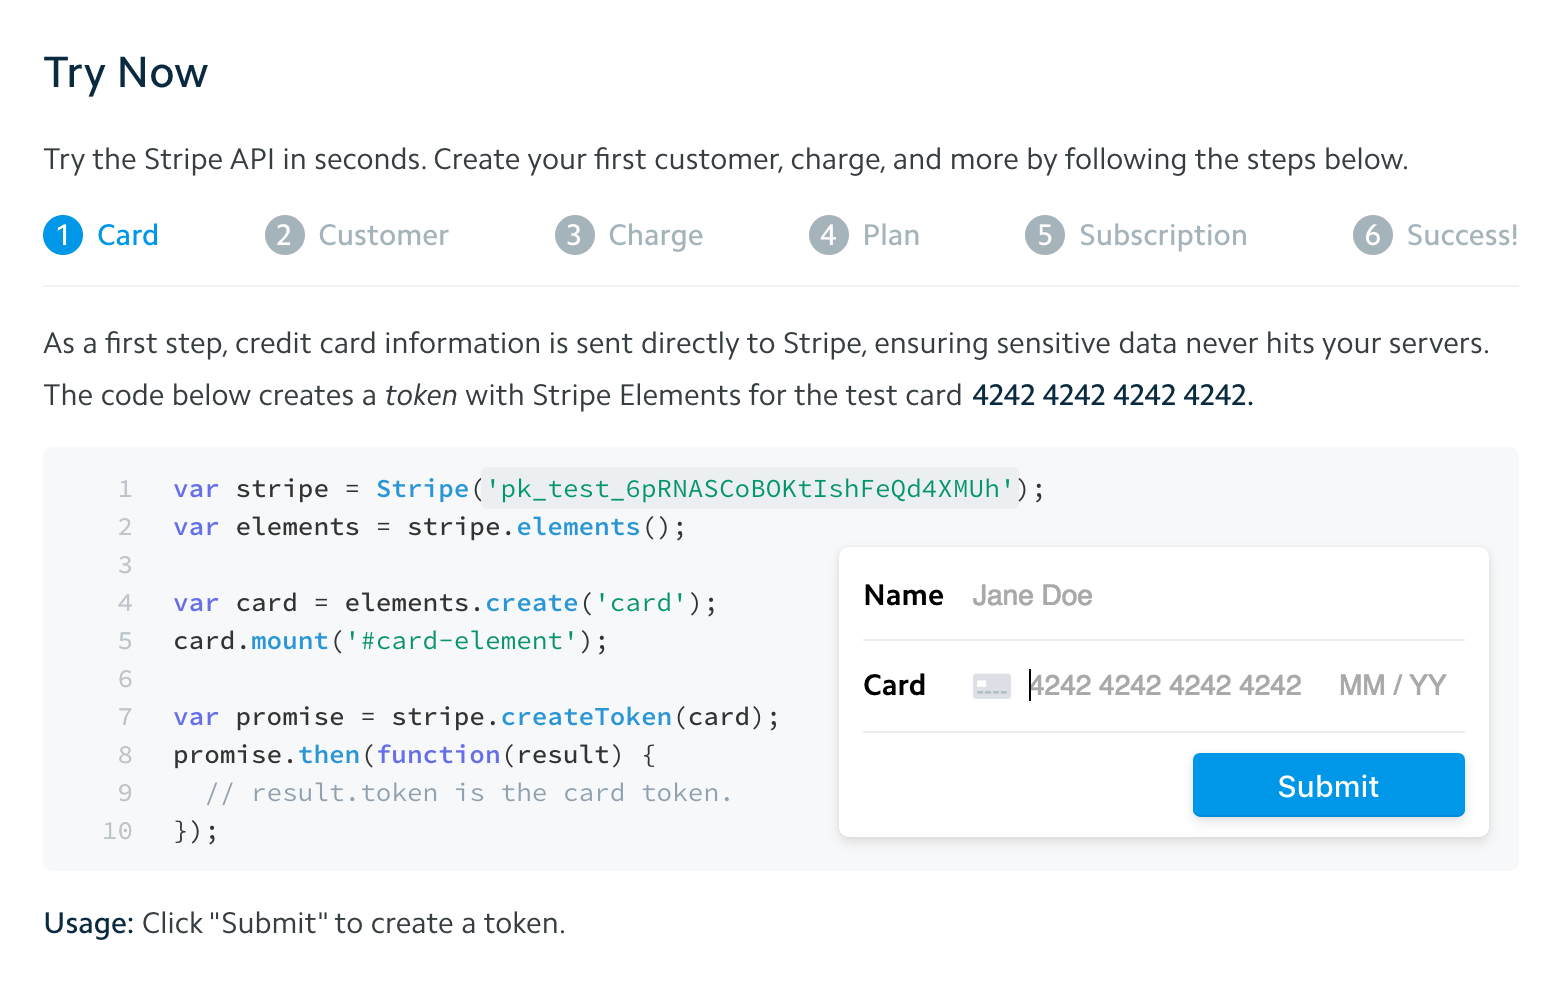
\includegraphics[scale=0.3]{stripe.png}
\caption{Stripe Api}
\label{fig:fig1}
\end{figure}

  \item \textbf{Paypal:}

  The PayPal APIs are HTTP-based RESTful APIs that use OAuth 2.0 for authorization. API request and response bodies are formatted in JSON.

\begin{figure}[!ht]\centering
\includegraphics[scale=0.3]{PayPal.png}
\caption{PayPal Api}
\label{fig:fig1}
\end{figure}
\newpage
\item \textbf{Twint:}

Twint is the closest implementation to Flouci, it offers payments through QR code scans.

The plugin allows QR code generation on the web page, it also creates a code for each transaction, It serves to confirm payments.
\begin{figure}[!ht]\centering
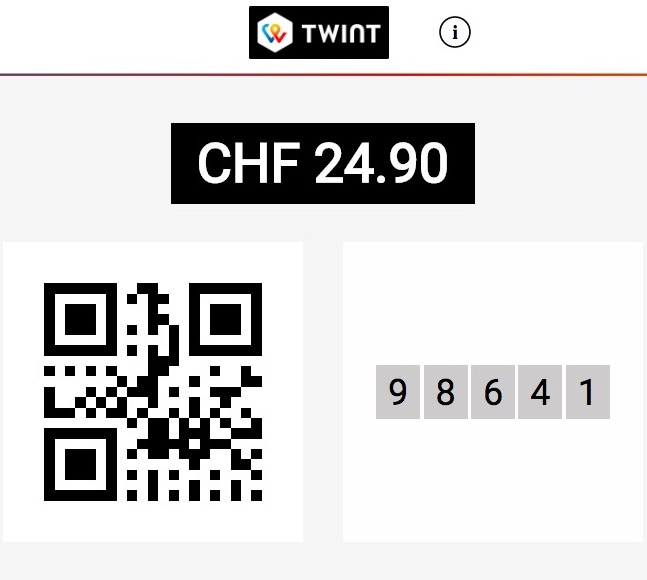
\includegraphics[scale=0.3]{twint.jpg}
\caption{Twint Pop-up}
\label{fig:fig1}
\end{figure}
  \end{itemize}
  
  

\section{Requirements specification}
A good in-depth requirements specification is the key to a solid foundation of any project.
The motivation behind this section is to take a global look at the project and be able to understand all the requirements needed to achieve our goals.
\subsection{Actors identification}
Actors are any entity that plays a role in our system. They can be users or systems that interact with our system. We were able to identify the external and internal actors of our platform. 
\newline
Among the internal actors we find:
\begin{itemize}
  \item \textbf{Anonymous Developer:} He can navigate on all the public pages of the site which are
accessible without authentication including the documentation part. Also, he can register a developer account.
  \item \textbf{Registred Developer:} He can manage his account, create and manage app's and integrate them on e-commerce websites.
  \item \textbf{Flouci User:}  He can use the checkout API the pay online merchants.
\end{itemize}
The external actors who are necessary for our platform are:
\begin{itemize}
  \item \textbf{Wallets API:} Is needed to activate any app. The app should be linked to a Flouci wallet.
  \item \textbf{Payments API:} Is needed for online payments.
\end{itemize}
\subsection{Functional requirements}
In this section, we will understand the functional requirements of our project by studying the global use case of our system.
	\newline In the Figure \ref{fig:usecasediagram}, we showcase the \textbf{general use case diagram} and then with the Table \ref{tab:usecasediagram} we explain more in-depth the different use cases.
\begin{figure}[H]\centering
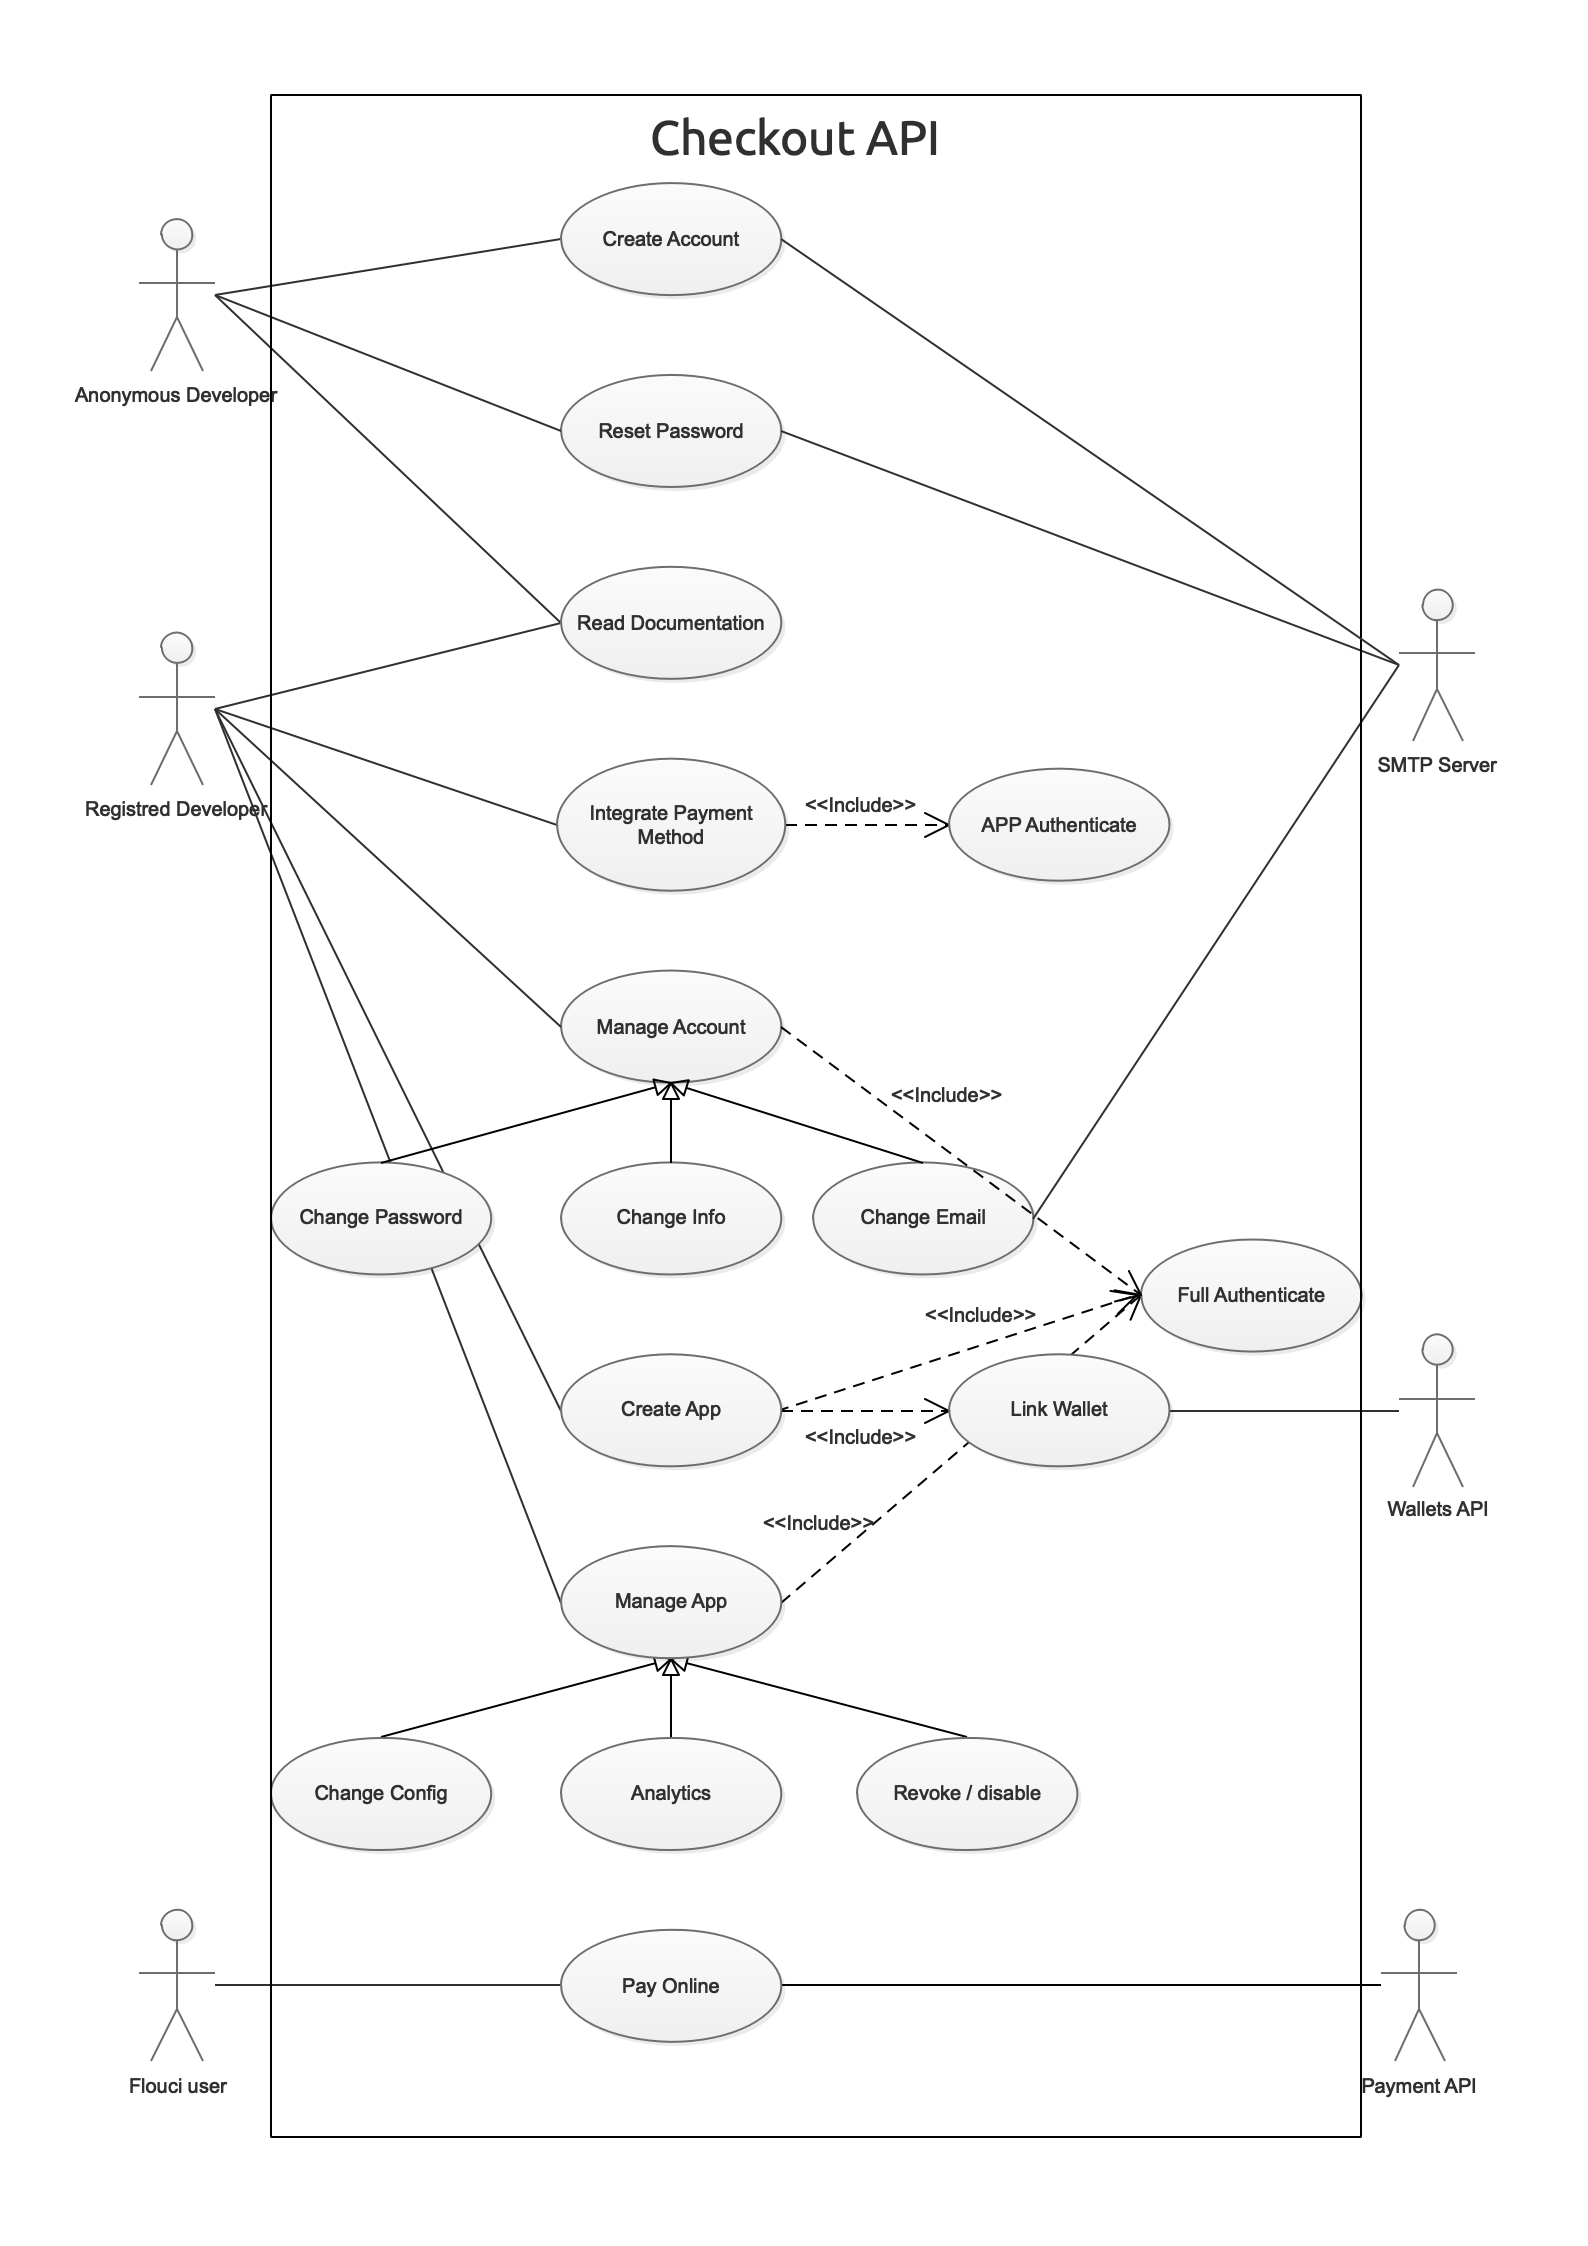
\includegraphics[scale=0.6]{GeneralUseCase.png}
\caption{General Use Case Diagram}
\label{fig:usecasediagram}
\end{figure}

\begin{table}[!h]
	\centering
	\caption{Use case description table}
	\footnotesize
	\begin{tabularx}
	{\linewidth}{|>{\centering{}\vspace*{\fill}}X|>{\centering{}\vspace*{\fill}}X|>{\vspace*{\fill}}X<{\centering{}}|}	
			\hline 
			 \bfseries Internal actor & \bfseries Use case &\bfseries External actor \\
			\hline 
			\multirow{3}{*}{Anonymous Developer}			&	Create Account: Any person with an email account can register for a Flouci developer account. 	&	SMTP Server			\\
			\cline{2-3}
				& Reset Password: In case a registered user forgets his password, he can reset it using his email address. 		&		SMTP Server		\\
				\cline{2-3}
					&	Read Documentation: Any person with access to the developer's platform can access the documentation.	&				\\
			\hline 
			\multirow{5}{*}{Registred Developer}					&	Read Documentation: The developer can access the documentation 	&				\\
			\cline{2-3}
			&	Integrate Payment Method: Any active app could be integrated into a commerce website and the integration only requires the public and private app tokens (App Authentication).	&				\\
			\cline{2-3}
					&	Manage Account:    The developer can change manage his account by changing his password, email or his basic info.	&		SMTP Server	\\
					\cline{2-3}
					&	Create App: An Authenticated developer can create an app and link it to a wallet with OTP verification through the Wallets API.	&			Wallets API	\\
					\cline{2-3}
					&	Manage App:	 An Authenticated  developer can check the analytics of his apps as well as tweak any app settings. &				\\		
					
			\hline 
			Flouci User	& Pay Online : With the pay with Flouci button on e-commerce websites, the Flouci user can quickly pay online merchants.  	&	Payment API	\\
			
			\hline
	\end{tabularx}
	\label{tab:usecasediagram}
\end{table}


\subsection{Non-functional requirements}
\subsubsection{Security}
When it comes to payment solutions security is the number one requirement to keep in mind.
Our solution implements many layers of security including: 
\begin{itemize}
	\item \textbf{HTTPS:} The platform only works on https mode, we use "Kaoun" trusted certificate.
	\item \textbf{JWT Token\cite{JWT}:}  Access to the platform is secured with JWT tokens, managing apps is only possible with this token.
	\item \textbf{Private / Public Tokens for Apps:}  In order to accept Payments Flouci user sign payments attached to the app public key and the developer can only accept them if he has the private key.
	App public keys can be revoked.
\end{itemize}
\subsubsection{Documentation}
An API is only usable with proper documentation, So in order to get developers to implement our solutions, we should have easy and understandable documentation. The documentation is accessible in our platform.\subsubsection{Logging}
Our Solution is using "logstash" to forward logs to our ELK\cite{ELK} stack, different log levels are used and we implemented a lot of metrics and dashboards on our kibana.

\begin{figure}[H]\centering
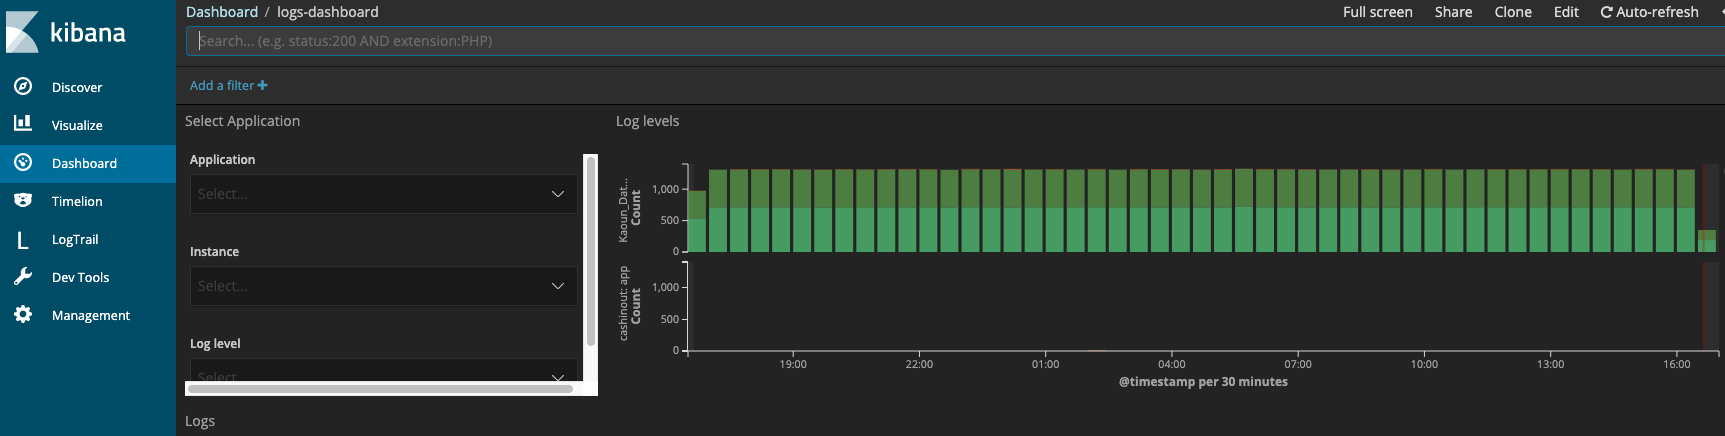
\includegraphics[scale=0.3]{ELK.png}
\caption{Kibana Dashboard}
\label{fig:usecasediagram}
\end{figure}

\subsubsection{Integrability}
Flouci online payment method can be easily integrated into any e-commerce website. It only requires an HTML form in the front end and an API call to accept payments on the backend.

\subsubsection{Extensibility}
Our payment method should allow extensibility and add more payment method other than the QR code scans. 
\subsubsection{Legal}
On the legal side, we should be compliant with the Tunisian laws and only enable appropriate users to accept payments.
This is achieved on the app creation level, at the stage of linking the wallet.
\subsubsection{Privacy}
Flouci users privacy should be considered at the highest levels, payment history and activities should be seen only by the persons with the right permissions.
\subsubsection{Ergonomics}
To guarantee a good control of our project and to simplify the interaction with the final users, we support our analysis of functional needs with mock-ups that model the different interfaces of our final product. These models are made by the "Adobe XD" tool and they are compliant with the overall Kaoun prouducts user experience. \newline Figure \ref{checkoutScreen} represents the checkout pop-up on e-commerce websites.
\newline Figure \ref{developersPlatform} represents the Developers API platform.

\begin{figure}[H]\centering
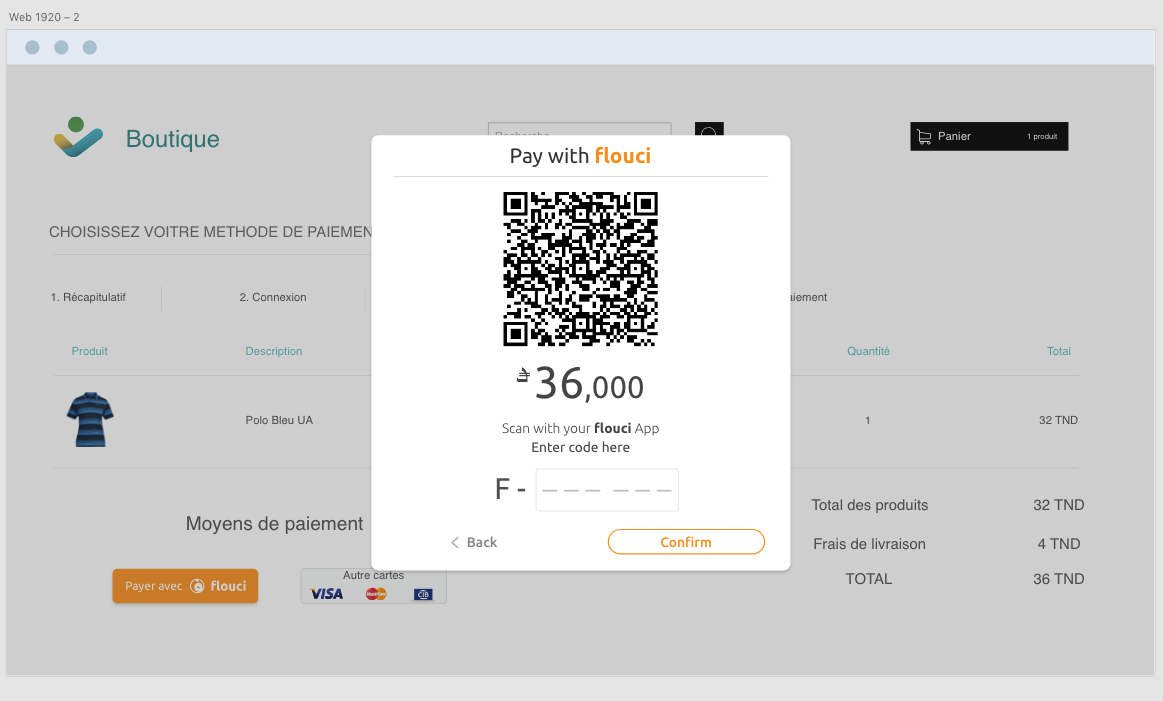
\includegraphics[scale=0.4]{Checkout_screen}
\caption{Checkout pop-up mock-up}
\label{checkoutScreen}
\end{figure}

\begin{figure}[H]\centering
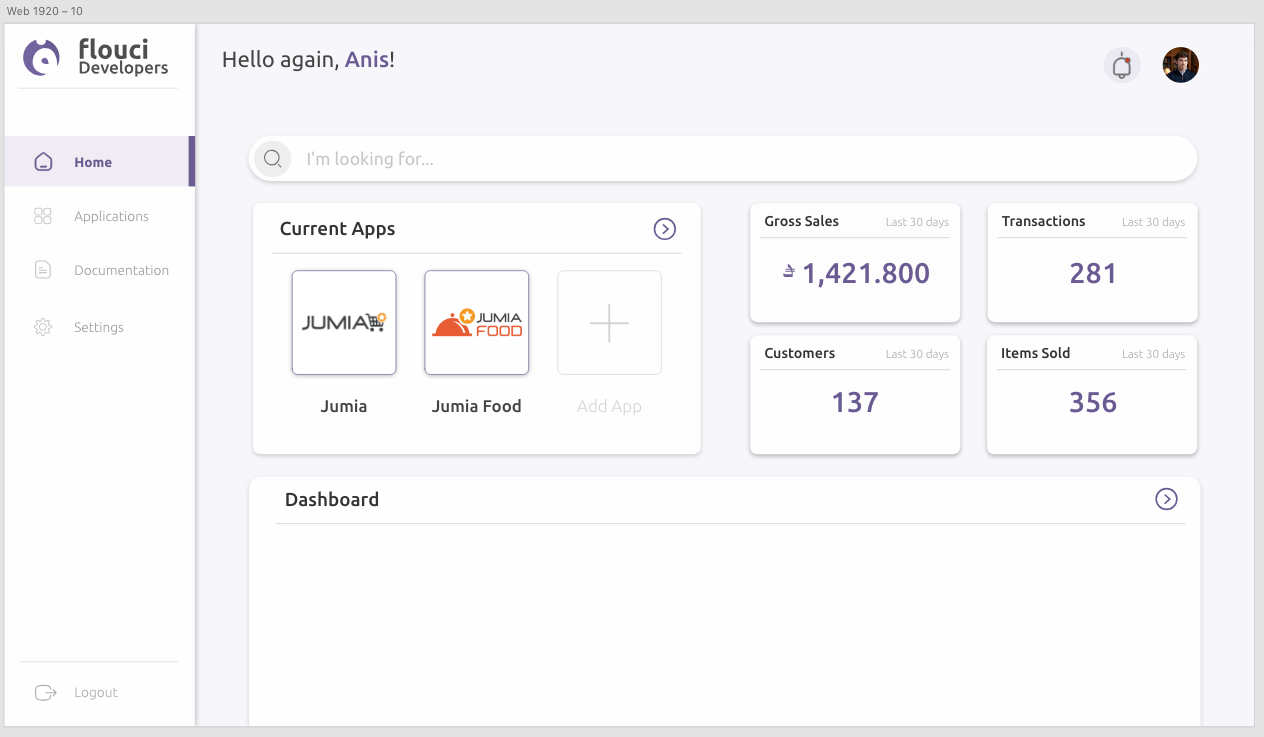
\includegraphics[scale=0.4]{web_screen}
\caption{Developers platform mock-up}
\label{developersPlatform}
\end{figure}

\section*{Conclusion}
In this chapter, we took the time to think about different aspects of our project, we went through detailed analysis in order to comprehend the project boundaries. After this we can launch our project development cycles which what we will be the topic of our next chapter.
%==============================================================================
\end{spacing}


\setcounter{chapter}{2}
\chapter{Realisation}
\minitoc %insert la minitoc
\graphicspath{{Chapitre3/figures/}}

%\DoPToC
%==============================================================================
\pagestyle{fancy}
\fancyhf{}
\fancyhead[R]{\bfseries\rightmark}
\fancyfoot[R]{\thepage}
\renewcommand{\headrulewidth}{0.5pt}
\renewcommand{\footrulewidth}{0pt}
\renewcommand{\chaptermark}[1]{\markboth{\MakeUppercase{\chaptername~\thechapter. #1 }}{}}
\renewcommand{\sectionmark}[1]{\markright{\thechapter.\thesection~ #1}}

\begin{spacing}{1.2}

%==============================================================================
\section*{Introduction}
Ce chapitre porte sur la partie pratique ainsi que la bibliographie.

\section{Outils et langages utilises}
L'etude technique peut se trouver dans cette partie, comme elle peut etre faite en
parallele avec l'etude theorique (comme le suggere le modele 2TUP).
Dans cette partie, il faut essayer de convaincre le lecteur de vos choix en termes de
technologie. Un etat de l'art est souhaite ici, avec un comparatif, une synthese et un choix 
d'outils, meme tres brefs.
\section{Presentation de l'application}
Il est tout e fait normal que tout le monde attende cette partie pour coller e souhait toutes les images
correspondant aux interfaces diverses de l'application si chere e votre coeur, mais
abstenez vous! Il FAUT mettre des imprime ecrans, mais bien choisis, et surtout, il faut les scenariser : Choisissez un scenario d'execution, par exemple la creation d'un 
nouveau client, et montrer les differentes interfaces necessaires pour le faire, en
expliquant brievement le comportement de l'application. Pas trop d'images, ni trop de
commentaires : concis, encore et toujours.

evitez ici de coller du code : personne n'a envie de voir le contenu de vos classes.
Mais  vous  pouvez inserer des snippets (bouts de code) pour montrer certaines
fonctionnalites \cite{ELKALMEL2019}\cite{Latex}, si vous en avez vraiment besoin. Si vous voulez montrer une partie de votre code, les etapes d'installation ou de configuration, vous pourrez les mettre dans l'annexe.
\subsection{Exemple de tableau}

Vous pouvez utiliser une description tabulaire d'une eventuelle comparaison entre les travaux existants. Ceci est un exemple de tableau: Tab \ref{tab:exple}.

\begin{table}[ht]
	\centering
	\caption{Tableau comparatif}
	\footnotesize
	\begin{tabularx}{\linewidth}{|>{\bfseries \vspace*{\fill}}X ||>{\centering{}\vspace*{\fill}}X|>{\centering{}\vspace*{\fill}}X|>{\centering{}\vspace*{\fill}}X|>{\vspace*{\fill}}X<{\centering{}}|}	
			\hline 
			& \bfseries Col1 & \bfseries Col2 &\bfseries Col3 &\bfseries Col4\\
			\hline \hline
			Row1		&		&	X	&		&		\\
			Row2		&	X	&		&		&		\\
			Row3		&	X	&	X	&	X	&	X	\\
			Row4		&	X	&		&	X	&	X	\\
			Row5		&	X	&		&	X	&	X	\\
			Row6		&	X	&		&	X	&	X	\\
			Row7		&	X	&		&	X	&		\\
			Row8		&	X	&	X	&	X	&		\\
			\hline
	\end{tabularx}
	\label{tab:exple}
\end{table}

\subsection{Exemple de Code}
Voici un exemple de code Java, avec coloration syntaxique \ref{code:java}.

\begin{lstlisting}[rulecolor=\color{white}]
\end{lstlisting}

\begin{lstlisting}[label=code:java,caption=Helloworld Java,language=java]
	public class HelloWorld {
	//la methode main
    public static void main(String[] args) {
        System.out.println("Hello, World");
    }

}
\end{lstlisting}

\section{Remarques sur la bibliographie}
Votre bibliographie doit repondre e certains criteres, sinon, on vous fera encore et
toujours la remarque dessus (et parfois, meme si vous pensez avoir tout fait comme il
 faut, on peut vous faire la remarque quand meme : chacun a une conception tres
personnelle de comment une bibliographie devrait etre).\\
\begin{itemize}
\item Une bibliographie dans un bon rapport doit contenir plus de livres et d'articles 
que de sites web : apres tout c'est une biblio. Privilegiez donc les ouvrages
reconnus et publies pour vos definitions, au lieu de sauter directement sur le premier article wikipedia;
 \item Les elements d'une bibliographie sont de preference classes par ordre
alphabetique, ou par themes (et ordre alphabetique pour chaque theme);
\item Une entree bibliographique doit etre sous la forme suivante :
\begin{itemize}
\item Elle doit contenir un identifiant unique: represente soit par un numero
[1] ou par le nom du premier auteur, suivi de l'annee d'edition [Kuntz, 1987];
\item Si c'est un livre : Les noms des auteurs, suivi du titre du livre, de l'editeur, 
ISBN/ISSN, et la date d'edition;
\item Si c'est un article : Les noms des auteurs, le titre , le journal ou la
conference, et la date de publication;
\item Si c'est un site web ou un document electronique : Le titre, le lien et la date 
de consultation;
\item Si c'est une these : nom et prenom, titre de la these, universite de
soutenance, annee de soutenance, nombre de pages;
\item Exemples : 
\begin{description}
\item $[Bazin, 1992]$ BAZIN R., REGNIER B. Les traitements antiviraux et leurs essais
therapeutiques. Rev. Prat., 1992, 42, 2, p.148-153.\\
\item $[Anderson,1998]$ ANDERSON P.JF. Checklist of criteria used for evaluation of metasites.
[en ligne]. Universite du Michigan, Etats Unis. Site disponible sur :\\
http://www.lib.umich.edu/megasite/critlist.html.(Page consultee le 11/09/1998).
\end{description}
\item Dans le texte du rapport, on doit obligatoirement citer la reference en  faisant appel e son identifiant, juste apres avoir utilise la citation. Si ceci n'est pas fait dans les regles, on peut etre accuse de plagiat.
\end{itemize} 
\end{itemize} 

\section*{Conclusion}
Voile.

%==============================================================================
\end{spacing}


\backmatter
\pagestyle{fancy}
\fancyhf{}
\renewcommand{\chaptermark}[1]{\markboth{Conclusion Generale et Perspectives}{}}
\fancyhead[R]{Conclusion Generale et Perspectives}
\fancyfoot[R]{\thepage}
\renewcommand{\headrulewidth}{0.5pt}
\renewcommand{\footrulewidth}{0pt}
\chapter{General Conclusion and Perspectives }
%==============================================================================
\pagestyle{fancy}
\fancyhf{}
\fancyhead[R]{\bfseries\rightmark}
\fancyfoot[R]{\thepage}
\renewcommand{\headrulewidth}{0.5pt}
\renewcommand{\footrulewidth}{0pt}
\renewcommand{\chaptermark}[1]{\markboth{\MakeUppercase{\chaptername~\thechapter. #1 }}{}}
\renewcommand{\sectionmark}[1]{\markright{\thechapter.\thesection~ #1}}

\begin{spacing}{1.2}
%==============================================================================
During a period of four months, we had to design and implement our challenging project. We needed to expand the Flouci ecosystem and add the ability to perform online integrations.
The project had to involve a lot of pieces, A platform that allows developers to manage their integration, A module that could be integrated into e-commerce websites, As well as the existing API's of The Flouci ecosystem including the payment API and the Wallets API.   

We started our work by setting up a modern software development discipline. We followed the Kanban methodology and created our project board from day one. We also defined a DevOps pipeline that involves different steps from testing to packaging and deploying. And we followed a strict TDD to ensure that we have a good testing coverage. 

Only after making sure that we can write code in the best quality possible and making the development experience as modern as we could that we started implementing our core functionalities. 

First, we started implementing the developer's platform, We challenged ourselves to build the front end in React, Since the company was shifting all its products to react and that's when we knew that in order to finish our product we needed to be adapt and learn anything.

After finishing our platform, we dived into the next sprint and started developing the integration module. The hardest part of the project was to make the module as portable as possible, and we had to make it in pure javascript.  

In the end, we delivered a platform to create integration apps, as well as a simple module that could use those apps to add the Flouci payment method on any website. It only takes the knowledge of performing a REST call to complete the integration.

From this state, our project could evolve and add more functionalities:
\begin{itemize}
	\item \textbf{Plateform:} We could add more customization to our integration app and allow developers to add their users and items. After that we can add more metrics relevant to items or users like most sold items, or most active customers.
	\item \textbf{Checkout module:} we can add the possibility to pay with the Flouci login credentials, and also we can make a button that redirects to the app on mobile devices to perform payments without having to scan any QR codes.
\end{itemize} 

%==============================================================================
\end{spacing}

\bibliographystyle{Biblio/unsrt_modif}
\singlespacing
\renewcommand{\bibname}{Bibliographique}

\bibliography{Biblio/aesm_edspia}

\onehalfspacing

\appendix
\setcounter{figure}{0} 
\setcounter{table}{0}
\setcounter{footnote}{0}
\setcounter{equation}{0}
\pagestyle{fancy}
\fancyhf{}
\renewcommand{\chaptermark}[1]{\markboth{\MakeUppercase{#1 }}{}}
\renewcommand{\sectionmark}[1]{\markright{\thesection~ #1}}
\fancyhead[RO]{\bfseries\rightmark}
\fancyhead[LE]{\bfseries\leftmark}
\fancyfoot[RO]{\thepage}
\fancyfoot[LE]{\thepage}
\renewcommand{\headrulewidth}{0.5pt}
\renewcommand{\footrulewidth}{0pt}

\makeatletter
\renewcommand\thefigure{A.\arabic{figure}}
\renewcommand\thetable{A.\arabic{table}} 
\makeatother

\chapter{Annexe : Remarques Diverses}
\graphicspath{{Annexe1/figures/}}
%==========================================================================

%    Annexe

%===========================================================================
\begin{itemize}
\item Un rapport doit toujours �tre bien num�rot�;
\item De pr�f�rence, ne pas utiliser plus que deux couleurs, ni un caract�re fantaisiste; 
\item Essayer de toujours garder votre rapport sobre et professionnel; 
\item Ne jamais utiliser de je ni de on, mais toujours le nous (m�me si tu as tout fait tout seul); 
\item Si on n'a pas de paragraphe 1.2, ne pas mettre de 1.1;
\item TOUJOURS, TOUJOURS faire relire votre rapport � quelqu'un d'autre (de pr�f�rence qui n'est pas du domaine) pour vous corriger les fautes d'orthographe et de fran�ais;
\item Toujours valoriser votre travail : votre contribution doit �tre bien claire et mise en �vidence; 
\item Dans chaque chapitre, on doit trouver une introduction et une conclusion;
\item Ayez toujours un fil conducteur dans votre rapport. Il faut que le lecteur suive un raisonnement bien clair, et trouve la relation entre les diff�rentes parties;
\item Il faut toujours que les abr�viations soient d�finies au moins la premi�re fois o� elles sont utilis�es. Si vous en avez beaucoup, utilisez un glossaire.
\item Vous avez tendance, en d�crivant  l'environnement mat�riel, � parler de votre ordinateur, sur lequel vous avez d�velopp� : ceci est inutile. Dans cette partie, on ne cite que le mat�riel qui a une influence sur votre application. Que vous l'ayez d�velopp� sur Windows Vista ou sur Ubuntu n'a aucune importance;
\item Ne jamais mettre de titres en fin de page; 
\item Essayer toujours d'utiliser des termes fran�ais, et �viter l'anglicisme. Si certains termes  sont plus connus en  anglais, donner leur �quivalent en fran�ais la premi�re fois que vous les utilisez, puis utilisez le mot anglais, mais en italique;
\item �viter les phrases trop longues : clair et concis, c'est la r�gle g�n�rale !\\

\newpage

\textbf{Rappelez vous que votre rapport est le visage de votre travail : un mauvais rapport peut �clipser de l'excellent travail. Alors pr�tez-y l'attention n�cessaire.}

 
\begin{figure}[!ht]\centering

\includegraphics[scale=0.5]{ingenieur.jpg}
\end{figure}
\end{itemize}



\end{document}
